\subsection{Word embedding}\label{chap:background:we}

Word embeddings or distributional vectors can be seen as a way of representing words. They follows the distributional hypothesis, that words with similar meanings tend to appear in similar contexts. They capture the characteristics of words in a corpus, thus having an advantage of capturing similarity between words which can be computed using the cosine similarity measure. They are often used as a resource, allowing the creation of NLP applications capable of understanding textual analogies even with few data for training. They are widely used for NLP in the last years. \cite{DBLP:journals/corr/abs-1708-02709, Harris1954, Hartmann2017}.


In many traditional NLP applications, \textbf{one-hot vectors}, shown in \autoref{fig:vectors}, were used to represent words of a vocabulary. In this case, we have a vector for each word of the vocabulary with the same size, filled with zeros beside the position of the word where we have the value one \cite{turian2010word}.
One problem of using the one-hot representation is that you can't generalize crosswords because of the inner product of any 1-hot vector is always zero. And for this reason, we cannot apply any distance-like metrics to evaluate the similarity. For this reason, a \textbf{feature vector} is preferable to word representation. In this case, we have for each word an vector of size $d$ filled with real values between 0 and 1 that represents multiple features. There are several ways to learn these high dimensional feature vectors values. \cite{turian2010word}.

\begin{figure}[h]
	\caption{One-hot versus feature vectors.}
	\label{fig:vectors}
	\centering%
	\begin{minipage}{.7\textwidth}
		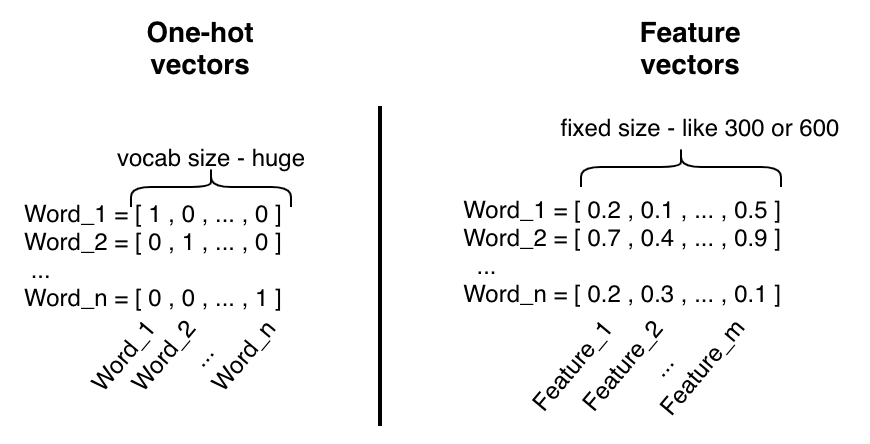
\includegraphics[width=\textwidth]{vectors.png}
		\fonte{Made by the author.}
	\end{minipage}
\end{figure}


These feature vectors or embeddings can be generated using neural networks. \citetexto{Bengio:2003} first introduced the term word embeddings with a simple feed forward neural language model to learn these vectors. After this, other models emerged with the creation of a toolkit named \textit{word2vec} presented by \citetexto{Mikolov2013DistributedRO}.

\textbf{Word2vec} is a predictive embedding model composed by two main architectures to produce word embeddings, as shown in \autoref{fig:word2vec}:

\begin{itemize}
    \item \textbf{Continuous bag-of-words} (CBOW): Learns the embedding by predicting the current word based on their surrounding words (context).
    \item \textbf{Skip-gram} (SG): It is the opposite of CBOW, it learns by predicting the surrounding words (context) given a current word.
\end{itemize}

\begin{figure}[h]
	\caption{Word2Vec training architectures.}
	\label{fig:word2vec}
	\centering%
	\begin{minipage}{.9\textwidth}
		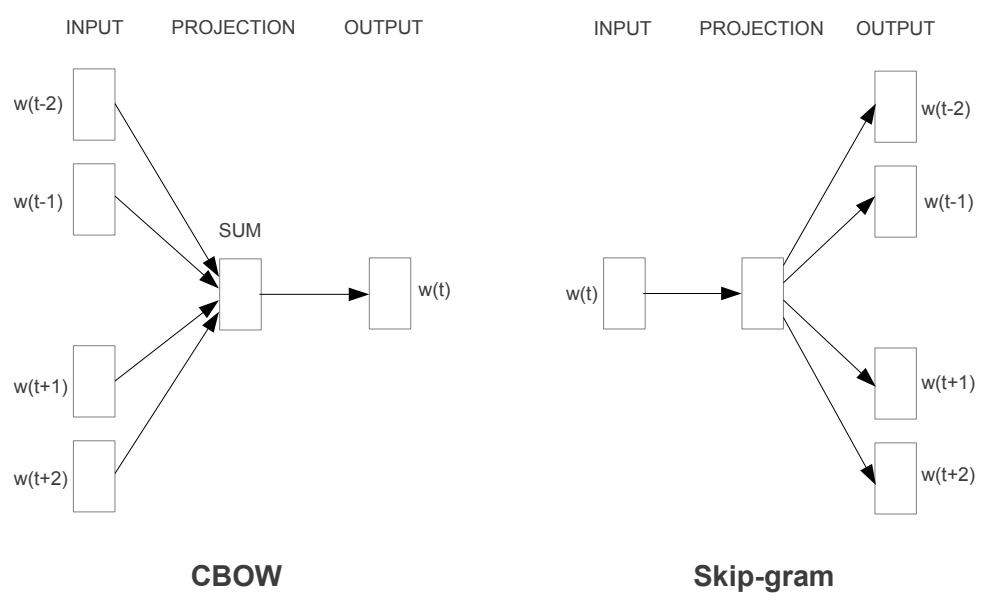
\includegraphics[width=\textwidth]{word2vec.png}
		\fonte{Taken from \citetexto[p.~5]{DBLP:journals/corr/abs-1301-3781}.}
	\end{minipage}
\end{figure}

After word2vec other algorithms emerged, such as \textbf{Global Vectors} (GloVe). \citetexto{Pennington2014} describes their work as "GloVe, is a new global log-bilinear regression model for the unsupervised learning of word representations that outperforms other models on word analogy, word similarity, and named entity recognition tasks.". GloVe is an approach that combines the global statistics of matrix factorization with the context based learning from word2vec.

\citetexto{Ling:2015:naacl} presents \textbf{Wang2vec} an extensions of the original word2vec models to improve the embeddings obtained for syntactically motivated tasks, by introducing changes that made the network aware of the relative positioning of context words.

Later on, \citetexto{bojanowski2016enriching} introduces \textbf{FastText}, which is another way to learn word representations by taking into account subword information. They incorporate character $n$-grams into the Skip-Gram model. By their evaluation the model outperforms baselines that do not take into account subword information.

% --------------------------

% The other family of word embedding model learns semantics by passing a window over the corpus line-by-line and learning to predict either the surroundings of a given word (Skip-gram model), or predict a word given its surroundings (continuous bag-of-words model). Note the bag-of-words problem is often shortened to “CBOW”.

% According to Mikolov et at., the authors of the word2vec paper, the two approaches differ slightly in performance:

% Skip-gram: works well with small amount of the training data, represents well even rare words or phrases.
% CBOW: several times faster to train than the skip-gram, slightly better accuracy for the frequent words.
% The authors of the GloVe paper note, however, that these context window-based methods suffer from the disadvantage of not learning from the global corpus statistics. As a result, repetition and large-scale patterns may not be learned as well with these models as they are with global matrix factorization. 